\documentclass[14pt]{article}

\usepackage[utf8x]{inputenc}
\usepackage[russian]{babel}
\usepackage{graphicx}
\graphicspath{{images/}}
\DeclareGraphicsExtensions{.pdf,.png,.jpg}

\usepackage{amsmath}
\usepackage{pgfplots}

\usepackage{geometry} % Меняем поля страницы
\geometry{left=2cm}% левое поле
\geometry{right=1.5cm}% правое поле
\geometry{top=2cm}% верхнее поле
\geometry{bottom=2cm}% нижнее поле

\renewcommand{\theenumi}{\arabic{enumi}}
\renewcommand{\labelenumi}{\arabic{enumi}}
\renewcommand{\theenumii}{.\arabic{enumii}}
\renewcommand{\labelenumii}{\arabic{enumi}.\arabic{enumii}.}
\renewcommand{\theenumiii}{.\arabic{enumiii}}
\renewcommand{\labelenumiii}{\arabic{enumi}.\arabic{enumii}.\arabic{enumiii}.}

\begin{document}
\begin{titlepage}
	\begin{center}
		\fontsize{18pt}{20pt}\selectfont
		\textbf{Работа 4.3.1.}	
	
		\vspace{5cm}
		\fontsize{24pt}{25pt}\selectfont
		Изучение дифракции света
	\end{center}
	\begin{flushright}
		\fontsize{18pt}{20pt}\selectfont
		\vspace{14cm}
		\hspace{-3cm}
		\textit{Корнеев Е.С.}
	\end{flushright}		
\end{titlepage}

\begin{center}
	\fontsize{16pt}{18pt}\selectfont	
	Изучение дифракции света
\end{center}


\fontsize{14pt}{16pt}\selectfont
\vspace{1cm}
\textbf{Цель работы:} изучение дифракции Френеля и Фраунгофера.

\vspace{0.5cm}
\textbf{Оборудование:} оптическая скамья, ртутная лампа, монохроматор, щели с регулируемой шириной, рамка с вертикальной нитью, двойная щель, микроскоп на поперечных салазках с микрометрическим винтом, зрительная труба.

\vspace{1cm}
\textbf{Дифракция Френеля}

Схема установки для наблюдения дифракции Френеля представлена на рис. 1. Световые лучи освещают щель $S2$ и испытывают на ней дифракцию. Дифракционная картина рассматривается с помощью микроскопа $M$, сфокусированного на некоторую плоскость наблюдения $\Pi$.

\begin{figure}[h!]
	\center{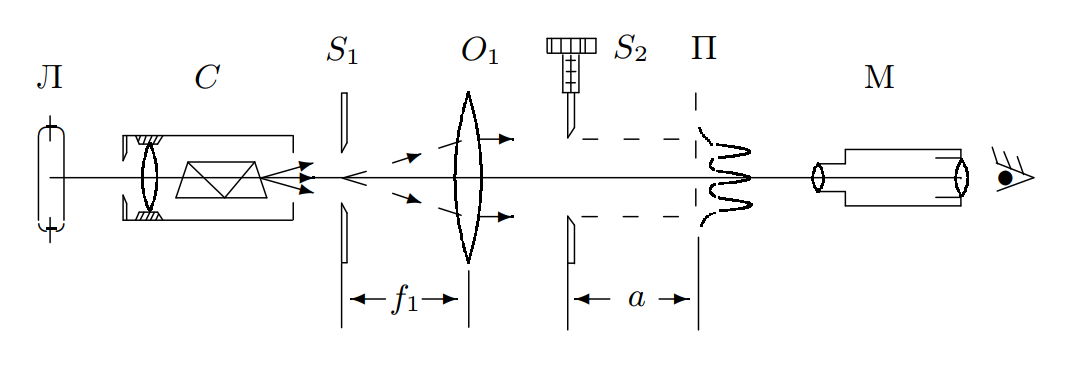
\includegraphics[width = 14cm]{1}}
	\caption{Схема установки для наблюдения дифракции Френеля}
	\label{fig:image}
\end{figure}

Щель $S2$ освещается параллельным пучком монохроматического света с помощью коллиматора, образованного объективом $O1$ и щелью $S1$, находящейся в его фокусе. На щель $S1$ сфокусировано изображение спектральной линии, выделенной из спектра ртутной лампы $Л$ при помощи простого монохроматора $C$, в котором используется призма прямого зрения. 

Распределение интенсивности света в плоскости наблюдения $\Pi$ проще всего рассчитывать с помощью зон Френеля (для щели их иногда называют зонами Шустера). При освещении щели $S2$ параллельным пучком лучей (плоская волна) зоны Френеля представляют собой полоски, параллельные краям щели (рис. 2). Результирующая амплитуда в точке наблюдения определяется суперпозицией колебаний от тех зон Френеля, которые не перекрыты створками щели. Графическое определение результирующей амплитуды производится с помощью векторной диаграммы -- спирали Корню. Суммарная ширина $m$ зон Френеля $z_m$ определяется соотношением
$$
	z_m = \sqrt{am\lambda}
$$

где
$a$ -- расстояние от щели до плоскости наблюдения (рис. 1), а $\lambda$ -- длина волны.

Вид наблюдаемой дифракционной картины определяется \textsl{числом Френеля} $\Phi$: квадрат числа Френеля
$$
	\Phi = \frac{D}{\sqrt{a\lambda}} ~-
$$

\begin{figure}[h!]
	\center{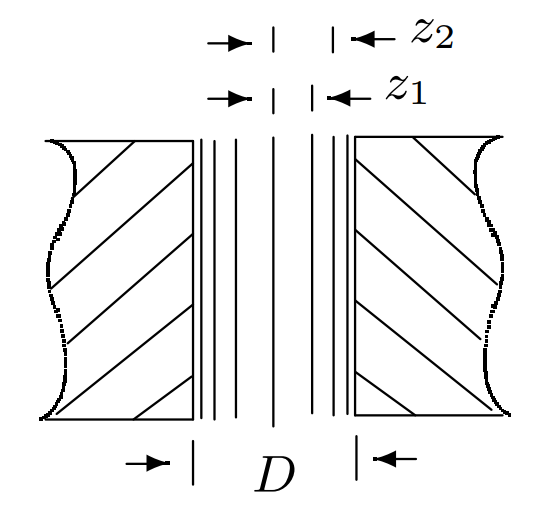
\includegraphics[width = 6cm]{2}}
	\caption{Зоны Френеля в плоскости щели}
	\label{fig:image}
\end{figure}

это отношение ширины щели $D$ к размеру первой зоны Френеля, т.е. число зон Френеля, которые укладываются на ширине щели. Обратную величину называют \textsl{волновым параметром}
$$
	p = \frac{1}{\Phi} = \frac{\sqrt{a\lambda}}{D}
$$

Дифракционная картина отсутствует, когда плоскость наблюдения $\Pi$ совпадает с плоскостью щели: при $\Phi \rightarrow \infty$ мы имеем дело с геометрической оптикой. При небольшом удалении от щели, когда число Френеля $\Phi \gg 1$ (на щели укладывается огромное число зон), распределение интенсивности света за щелью также можно получить с помощью законов геометрической оптики (приближённо). Дифракционная картина в этом случае наблюдается только в узкой области на границе света и тени у краёв экрана.

При последующем небольшом удалении от щели (или изменении ширины щели $S2$) эти две группы дифракционных полос перемещаются практически независимо друг от друга. Каждая из этих групп образует картину дифракции Френеля на краю экрана. Распределение интенсивности при дифракции света на краю экрана может быть найдено с помощью спирали Корню. 

При дальнейшем увеличении расстояния a (или уменьшении ширины щели $S2$) обе системы дифракционных полос постепенно сближаются и, наконец, при $\Phi \geq 1$ накладываются друг на друга. Распределение интенсивности в плоскости наблюдения в этом случае определяется числом зон Френеля, укладывающихся на полуширине щели. Если это число равно $m$, то в поле зрения наблюдается $n = m - 1$ тёмных полос. Таким образом, по виду дифракционной картины можно оценить число зон Френеля на полуширине щели.

\vspace{1cm}
Соберем схему согласно рис. 1.

Откроем щель, выставив ширину равную 0.30мм, используя микрометрический винт.

Добившись наибольшей чёткости дифракционной картины, найдем резкое изображение щели (чёткие края без дифракционных полос). Запишем начальное положение микроскопа -- координату по шкале продольной линейки, расположенной на оптической скамье. Тубус микроскопа закреплён на подставке с продольной шкалой, зафиксируем начальное положение микроскопа по этой шкале. Оно оказалось равно
$$
	L_0 = 50.0~\text{см}
$$

Постепенно отодвигая микроскоп от щели $S2$, заметим по шкале положение микроскопа, при котором на фоне щели видна одна тёмная полоса. Смещение микроскопа от первоначального положения даёт величину $z$ — расстояние от щели до плоскости наблюдения. 

Приближая микроскоп к щели, снимем зависимость координаты микроскопа $L$ от числа $n$ наблюдаемых тёмных полос и определим значение $z = L - L_0$:

\begin{center}
\begin{tabular}{|c|c|c|}
\hline
$m$	&	$L$, см	&	$z$, см	\\
\hline
1	&	52.7	&	2.7		\\
\hline
2	&	51.7	&	1.7		\\
\hline
3	&	51.1	&	1.1		\\
\hline
4	&	51.0	&	1.0		\\
\hline
5	&	50.9	&	0.9		\\
\hline
6	&	50.8	&	0.8		\\
\hline
\end{tabular}
\end{center}

При это погрешность определения $L$ и $L_0$ равна 1мм, откуда $\sigma_z = 2$мм.

Измерим ширину $b$ щели $S2$, используя микрометрический винт поперечных салазок микроскопа. Получим
$$
	b = 0.30 \text{мм},
$$
\noindent что совпадает с измеренным ранее значением. 

Получим:
\begin{center}
\begin{tabular}{|c|c|c|c|c|c|c|c|c|}
\hline
$n$					&	2		&	3		&	4		&	5		&	6		&	7		\\
\hline
$2\xi$, мм			&	0.24	&	0.27	&	0.27	&	0.30	&	0.31	&	0.31	\\
\hline
$\sigma_{2\xi}$,мм	&	0.02	&	0.03	&	0.05	&	0.06	&	0.07	&	0.08	\\
\hline
\end{tabular}
\end{center}

Погрешность $\sigma_{2\xi}$ определим считая $\xi = f(z)$:
$$
	\sigma_{2\xi} = \frac{\partial f}{\partial z}\sigma_z = \frac{\sigma_z}{\sqrt{nz\lambda}}
$$

Потроим график:
\begin{flushleft}
\begin{tikzpicture}
\begin{axis}[
	height = 9cm,
	width  = 15cm,
	every axis y label/.style={at = {(ticklabel cs: 0.5)}, rotate = 90, anchor = near ticklabel},
	xlabel = {$n$},
	ylabel = {$2\xi$, мм},
	xtick  = {2,...,7},
%	ytick  = {0.20,0.22,0.24,0.26,0.28,0.30,0.32},
	y tick label style={/pgf/number format/fixed zerofill}
]
\addplot+[
	only marks,
	error bars/.cd, 
	y dir = both, y explicit,
	x dir = both, x explicit,
	]
coordinates{
	(2, 0.24)	+- (0,0.02)
	(3, 0.27)	+- (0,0.02)
	(4, 0.27)	+- (0,0.02)
	(5, 0.30)	+- (0,0.02)
	(6, 0.31)	+- (0,0.02)
	(7, 0.31)	+- (0,0.02)	
};

\addplot [mark = none]
coordinates{
	(2, 0.3)
	(7, 0.3)
};

\end{axis}
\end{tikzpicture}
\end{flushleft}

\vspace{1cm}
\textbf{Дифракция Фраунгофера на щели}

На значительном удалении от щели, когда ширина щели становится значительно меньше ширины первой зоны Френеля, изображение щели размывается и возникает дифракционная картина, называемая дифракцией Фраунгофера.

Дифракционная картина наблюдается здесь в фокальной плоскости объектива O2. Каждому значению угла $\Theta$ соответствует в этой плоскости точка, отстоящая от оптической оси на расстоянии
$$
	x = f_2 \tg\Theta \approx f_2\Theta
$$

Поскольку объектив не вносит дополнительной разности хода между интерферирующими лучами (таутохронизм), в его фокальной плоскости наблюдается неискажённая дифракционная картина Фраунгофера. Эта картина соответствует бесконечно удалённой плоскости наблюдения.

\begin{figure}[h!]
	\center{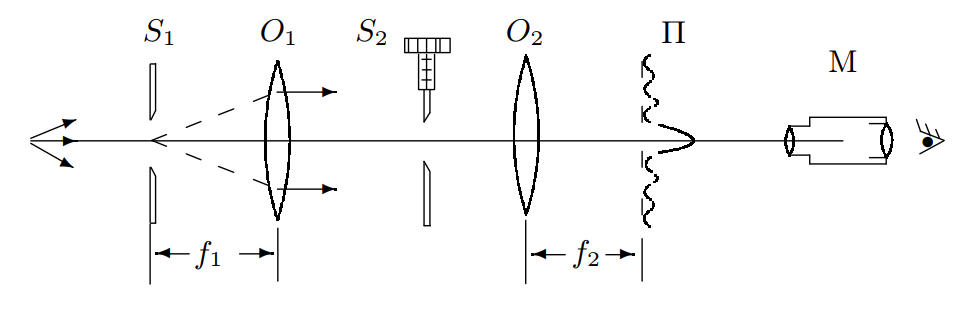
\includegraphics[width = 14cm]{4}}
	\caption{Схема установки для наблюдения дифракции Фраунгофера на щели}
	\label{fig:image}
\end{figure}

В центре поля зрения наблюдается дифракционный максимум (светлая полоса). При малых углах $\Theta$ положение минимумов (тёмных полос) определяется соотношением
$$
	\Theta_m = m\frac{\lambda}{b}
$$

Расстояние $x_m$ от тёмной полосы до оптической оси объектива O2 пропорционально фокусному расстоянию $f_2$. Из формул следует
$$
	x_m = m\frac{\lambda}{b}f_2
$$
Из последнего видно, что при малых углах минимумы эквидистантны, а расстояния $\delta x$ между минимумами обратно пропорциональны ширине $b$ щели $S2$.

\vspace{1cm}
Измерим с помощью винта поперечного смещения микроскопа координаты $X_m$ нескольких дифракционных минимумов при ширине щели $b = 0.15$мм. Фокусное расстояние линзы $f_2 = 11.0$см.

\begin{center}
\begin{tabular}{|c|c|c|}
\hline
$m$	&	$X_m$, мм	\\
\hline
-4	&	-1.16	\\ % 30
\hline
-3	&	-0.88	\\ % 32
\hline
-2	&	-0.58	\\ % 31
\hline
-1	&	-0.26	\\ % 33
\hline
1	&	0.38	\\ % 32
\hline
2	&	0.70	\\ % 34
\hline
3	&	1.06	\\ % 30
\hline
4	&	1.36	\\
\hline
\end{tabular}
\end{center}

Погрешность $X_m$ связана с приборной прогрешностью и равна 0.02мм.

Теперь можно построить график:

\begin{flushleft}
\begin{tikzpicture}
\begin{axis}[
	height = 9cm,
	width  = 15cm,
	every axis y label/.style={at = {(ticklabel cs: 0.5)}, rotate = 90, anchor = near ticklabel},
	xlabel = {$m$},
	ylabel = {$X_m$, мм},
	xtick  = {-4,...,4},
%	ytick  = {0.20,0.22,0.24,0.26,0.28,0.30,0.32},
	y tick label style={/pgf/number format/fixed zerofill}
]
\addplot+[
	only marks,
	error bars/.cd, 
	y dir = both, y explicit,
	x dir = both, x explicit,
	]
coordinates{
	(-4,-1.16)	+-	(0,0.02)
	(-3,-0.88)	+-	(0,0.02)
	(-2,-0.58)	+-	(0,0.02)
	(-1,-0.26)	+-	(0,0.02)
	( 1, 0.38)	+-	(0,0.02)
	( 2, 0.70)	+-	(0,0.02)
	( 3, 1.06)	+-	(0,0.02)
	( 4, 1.36)	+-	(0,0.02)
};

\addplot [mark = none, color = blue]
coordinates{
	(-4, -1.19583)
	(4, 1.35083)
};

\end{axis}
\end{tikzpicture}
\end{flushleft}

Найдем угловой коэффициент:
$$
	k = 0.32~\text{мм}
$$
Случайную погрешность определим по МНК:
$$
	\sigma_{k\text{случ}} = 0.01~\text{мм}
$$
Приборную определим, считая $k = f(X_m)$:
$$
	\sigma_{k\text{приб}} = \frac{\partial f}{\partial X_m}\sigma_{X_m} = 0.02~\text{мм}
$$
Откуда в итоге получается:
$$
	k = (0.32 \pm 0.02)~\text{мм}
$$
Среднее расстояние между минимумами численно равно $k$.

Теперь, зная, что
$$
	k = \frac{\lambda}{b}\cdot f_2~\Rightarrow~ b = \frac{\lambda f_2}{k}
$$
Получим
$$
	b = (0.18 \pm 0.01)~\text{мм}
$$
Заметим, что полученную величину можно считать совпадающей с измеренной напрямую шириной в пределах погрешности. 

\vspace{1cm}
\textbf{Дифракция Фраунгофера на двух щелях}

Для наблюдения дифракции Фраунгофера на двух щелях в установке следует заменить щель $S2$ экраном Э с двумя щелями. При этом для оценки влияния ширины входной щели на чёткость дифракционной картины вместо входной щели $S1$ следует поставить щель с микрометрическим винтом. Два дифракционных изображения входной щели, одно из которых образовано лучами, прошедшими через левую, а другое — через правую щели, накладываются друг на друга.

\begin{figure}[h!]
	\center{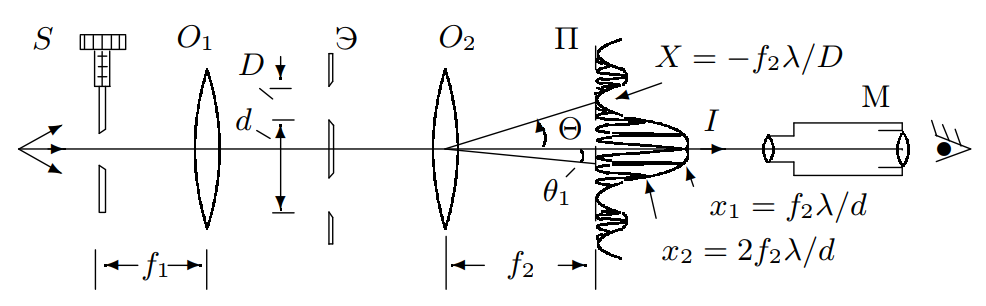
\includegraphics[width = 14cm]{5}}
	\caption{Схема установки для наблюдения дифракции Фраунгофера на двух щелях}
	\label{fig:image}
\end{figure}

Угловая координата $\Theta_m$ интерференционного максимума $m$-го порядка определяется соотношением
$$
	\Theta_m = m\frac{\lambda}{d}
$$
где $d$ -- расстояние между щелями. Линейное расстояние $\delta x$ между соседними интерференционными полосами в плоскости П равно, поэтому
$$
	\delta x = \frac{\lambda}{d}f_2
$$

Нетрудно оценить число $n$ интерференционных полос, укладывающихся в области центрального дифракционного максимума. Полная ширина главного максимума равна $2f_2\lambda/d$, где $b$ -- ширина щели, отсюда
$$
	n = \frac{2\lambda f_2}{b}\frac{1}{\delta x} = \frac{2d}{b}
$$

При дифракции света на двух щелях чёткая система интерференционных полос наблюдается только при достаточно узкой ширине входной щели S, которую можно рассматривать как протяжённый источник света размером $b$. Для наблюдения интерференции необходимо, чтобы расстояние $d$ между щелями не превышало радиуса когерентности
$$
	d \leq \frac{\lambda}{b}f_1
$$
Здесь $b$ -- ширина входной щели S и, следовательно, $b/f_1$ -- её угловая ширина. Таким образом, по размытию интерференционной картины можно оценить размер источника.

Не перемещая линз и микроскопа, заменим в установке входную щель S1 щелью с микрометрическим винтом и, слегка передвигая её вдоль скамьи, найдем в микроскопе резкое изображение новой входной щели. Поставим между линзами экран Э с двойной щелью. В области главного дифракционного максимума появится система равноотстоящих тёмных и светлых полос. Центрировкой системы и подбором ширины щели S добьемся наибольшей чёткости дифракционной картины.

Посчитаем число светлых промежутков между минимумами, лежащими в пределах главного максимума. Получим $n = 14$.

Измерим ширину центрального максимума: $L = 0.46$ мм. %0.46

Исследуйем влияние пространственной когерентности на видность интерференционной картины. Для этого, расширяя входную щель S, подберем такую ширину щели $b_0$, при которой наступает первое исчезновение интерференционных полос: $b_0 = 0.045$ мм. При этом ширина, при которой картина наиболее контрастна, равна 0.015 мм.

Теперь определим координаты границ щели:
\begin{center}
\begin{tabular}{|c|c|c|c|c|c|c|c|c|c|c|}
\hline
$x_1$, мм	&	$x_2$, мм	&	$x_3$, мм	&	$x_4$, мм	\\
\hline
0.40		&	0.64		&	2.20		&	2.46		\\
\hline
\end{tabular}
\end{center}

Погрешность $x_n$ примем равной приборной, т.е. 0.02 мм.

Отсюда
$$
	d = (156 \pm 4)\cdot10^{-2}\text{мм},
$$
$$
	b = (25 \pm 4)\cdot10^{-2}\text{мм}
$$
По формуле определим теорметическое число полос внутри максимума:
$$
	n = \frac{2d}{b} = 12,
$$
что хорошо согласуется с измеренным.

Также найдем $\delta x$:
$$
	\delta x = \frac{L}{n}
$$
откуда
$$
	x = (38 \pm 3)\cdot10^{-3}~\text{мм}
$$

Теперь можем определить теоретическое значение $d$:
$$
	\delta x = \frac{\lambda}{d}f_2 \Rightarrow d = \frac{f_2\lambda}{\delta x}
$$
$$
	d = (1.50 \pm 0.12)~\text{мм}
$$
Что совпадает с измеренным напрямую.

Также оценим $b_0$ из соотношения
$$
	\frac{\lambda}{b_0} \approx \frac{d}{f_1}~\Rightarrow~ b_0 \approx \frac{\lambda f_1}{d}
$$
Откуда
$$
	b_0 = 0.04~\text{мм}
$$
Видно, это эта величина близка к измеренной напрямую. 

\newpage
Таким образом, в данной лабораторной работе мы изучили дифракцию Френеля и Фраунгофера на щели и дифракцию Фраунгофера на двух щелях. 








\end{document}